\documentclass[11pt]{article}
\usepackage[margin=1in]{geometry}
\usepackage{amsmath,amssymb,amsfonts,bm}
\usepackage{booktabs}
\usepackage{multirow}
\usepackage{graphicx}
\usepackage{hyperref}
\usepackage{enumitem}
\usepackage{mathtools}
\usepackage{url}
\usepackage{tikz}
\usetikzlibrary{arrows.meta,positioning,shapes.geometric,calc,fit,backgrounds}
\usepackage{xcolor}
\hypersetup{colorlinks=true, linkcolor=blue, citecolor=blue, urlcolor=blue}

% placeholder macro for unfilled experimental numbers (will become a real number once experiments are run)
\newcommand{\TBD}{\textcolor{red!70!black}{\textbf{--}}}

\title{TrajCamo: Long-Window Trajectory Grouping Brings Video Reasoning Segmentation to Camouflaged Targets}
\author{}
\date{}

\begin{document}
\maketitle



\begin{abstract}
	We introduce \textbf{TrajCamo}, a language-guided video segmentation framework for camouflaged video object segmentation under implicit textual queries.
	Existing video reasoning segmentation methods rely on appearance-grounded tokens decoded from a few keyframes, which becomes fragile in camouflaged videos where the target is, by design, indistinguishable from its surroundings in any single frame.
	Prior camouflaged video methods compensate by exploiting motion, yet they all treat motion as an \emph{instantaneous} quantity --- a per-frame flow vector or a short-window correlation --- and are therefore easily confused by repetitive background dynamics such as flowing water, swaying foliage, or wind-driven texture, whose short-window motion is just as strong as the target's.
	Our central observation is that the right level at which to read motion in camouflaged video is the \emph{long window}: a camouflaged target, no matter how well it blends in, must move as a single physical entity over time, so its constituent pixels share a long-window trajectory structure that the background, composed of independently fluctuating texture elements, does not reproduce.
	Based on this observation, TrajCamo reformulates camouflaged video segmentation as the discovery of a spatially connected, kinematically consistent trajectory cluster that aligns with the language query.
	Accordingly, we propose a \emph{Long-Window Trajectory Field} that extracts dense point trajectories with native occlusion handling across the entire video, and a \emph{Kinematic Signature Encoder} that maps each trajectory to a learned embedding summarizing its long-window motion pattern.
	On top of these embeddings, we introduce a \emph{Long-Window Trajectory Grouping} module that recovers candidate object hypotheses as spatially connected, kinematically consistent subspaces, and a \emph{Query-conditioned Agentic Cluster Refinement} module in which a multimodal language agent iteratively interacts with a promptable video segmentation model: at each step it observes the current mask hypothesis and emits one of four actions --- \textsc{Select} a cluster, \textsc{Add-Pos}/\textsc{Neg} a point prompt, or \textsc{Terminate} --- until it commits to a final mask sequence.
	By replacing the appearance-grounding paradigm with long-window trajectory grouping and agentic mask refinement, TrajCamo establishes a principled and language-aware framework for camouflaged video understanding, in which the trajectory field serves both as the discovery signal for the target and as the long-range memory for its propagation, while the language model contributes a short, externally inspectable reasoning trace that selects and corrects motion hypotheses against the query.
\end{abstract}





\section{Introduction}

Understanding videos according to human intent is a central ability for intelligent vision systems.
In many practical scenarios, the object of interest is not specified by a precise category name or an explicit appearance description, but by a higher-level instruction that may involve commonsense, temporal comparison, or contextual reasoning.
This setting has recently motivated \emph{Video Reasoning Segmentation} (VRS), also known as ReasonVOS, where the model is required to output a sequence of segmentation masks for a video conditioned on a natural-language query~\cite{visa}.
Compared with classical referring video object segmentation, VRS moves from direct reference to implicit reasoning.
The model must not only understand what the query means, but also determine where the target is and how it evolves over time.

Recent progress in multimodal large language models has made this direction increasingly promising.
Methods such as VideoLISA, ViLLa, and VRS-HQ show that language models can be used as more than text generators: they can serve as reasoning engines that produce token representations suitable for dense prediction in videos~\cite{videolisa,villa,vrshq}.
Despite differences in design, these methods share a common recipe.
They first identify informative frames or clips, then encode the query and video into specialized tokens, and finally decode masks and propagate them through time.
This line of work has substantially expanded the scope of video segmentation from explicit language grounding to richer forms of reasoning.

However, the operating assumption behind these methods is that the target remains visually grounded in at least part of the video.
Once the problem shifts to \emph{camouflaged video object segmentation}, this assumption is undermined at the most basic level.
By definition, a camouflaged target has been selected by evolution or by adversarial design to look like its surroundings, so its appearance statistics on any single frame are barely separable from those of the background~\cite{cod10k}.
Prior work in this area has therefore turned to motion as an auxiliary signal, on the intuition that movement temporarily disturbs the camouflage~\cite{sltnet,moca}.
Unfortunately, motion in natural scenes is itself unreliable: water ripples, swaying grass, wind-driven foliage, and ambient parallax all produce continual per-frame motion, often with magnitudes comparable to or larger than that of the camouflaged target.
SLT-Net explicitly recognizes that explicit optical flow is unstable in such scenes and resorts to implicit motion modeling~\cite{sltnet}, while OCLR studies how camouflage can be both constructed and broken under a layered representation~\cite{oclrv}.
What is shared by these methods is that motion is still treated as a per-frame quantity: a magnitude, a flow vector, or an instantaneous correlation.

In this work, we argue that the difficulty in camouflaged video understanding is not the absence of motion, but the \emph{temporal scope} at which motion is read.
A camouflaged target, no matter how well it blends in, must move as a single physical entity over time.
Its constituent pixels traverse trajectories that, taken jointly across a long window, occupy a small, spatially compact, and internally consistent subset of the trajectory field.
The background, in contrast, is composed of independently fluctuating texture elements, fluid-like surfaces, and rigid scene parts whose motion is locally just as strong as the target's, but does not assemble into a single long-window structure.
This is exactly the property captured by the Gestalt principle of common fate, and exploited by classical trajectory-based motion segmentation~\cite{broxmalik,ochs2014}; what is new is that we can now read it at scale.
Recent advances in dense point tracking, including TAP-Vid~\cite{tapvid}, TAPIR~\cite{tapir}, OmniMotion~\cite{omnimotion}, and especially CoTracker3 with its joint cross-track attention and native occlusion handling~\cite{cotracker3}, have made it practical to extract long-window, occlusion-aware trajectories on real videos.
Concurrently, Karazija et al.~\cite{karazija} have shown that supervising segmentation with the low-rank subspace structure of long trajectories yields strong motion-based grouping, and SegAnyMo~\cite{seganymo} has demonstrated that such trajectories can directly serve as point prompts to a promptable video segmentation model.
What is still missing is a framework that brings these observations to bear on camouflaged video reasoning segmentation, where the discovery of the target must be reconciled with an implicit natural-language query.

Based on this view, we propose \textbf{TrajCamo}, a framework that brings the reasoning-token pipeline of VRS into the camouflaged video setting by changing what is grounded and how.
Instead of grounding the query against per-frame appearance features that are by construction unreliable for camouflage, TrajCamo grounds it against \emph{trajectory clusters}: spatially compact groups of dense point trajectories whose long-window motion is internally consistent.
The role of the language model is then to choose which of several physically plausible motion hypotheses corresponds to the query, rather than to localize a target whose appearance gives almost nothing away.
This factorization is natural for camouflage: long-window motion supplies the \emph{where} that any single frame cannot, while language supplies the \emph{what} that motion alone cannot disambiguate.

Concretely, TrajCamo consists of four tightly connected components.
We begin with a \textbf{Long-Window Trajectory Field}, which uses a foundation point tracker to extract dense, occlusion-aware trajectories that span the whole video, providing a temporally global representation that does not collapse under short occlusions or weak appearance contrast.
On top of these trajectories, we introduce a \textbf{Kinematic Signature Encoder}, which maps each trajectory to a learned embedding summarizing its long-window motion pattern, taking as input both the raw velocity time series and three derived statistical descriptors (spectral profile, multi-scale autocorrelation, and local rigidity) and letting the encoder learn whichever combination is most discriminative for trajectory-level grouping.
We then build a \textbf{Long-Window Trajectory Grouping} module that constructs candidate object hypotheses as spatially connected, kinematically consistent subspaces, with both an internal consistency score and an external contrast score against the local background.
Finally, we adopt a \textbf{Query-conditioned Agentic Cluster Refinement} mechanism, in which a multimodal language agent interacts iteratively with a promptable video segmentation model: at each step the agent observes the language query, the candidate clusters, and the current mask hypothesis, and emits one of four discrete actions --- \textsc{Select} a cluster, \textsc{Add-Pos}/\textsc{Neg} a point prompt, or \textsc{Terminate} --- and SAM2 re-runs full-video propagation under the updated prompt stream until the agent commits to a final mask.

TrajCamo retains the overall spirit of recent VRS systems, namely reasoning with language and decoding masks through a promptable segmentation model.
At the same time, it changes the modeling assumption from \emph{appearance-grounded localization} to \emph{long-window trajectory grouping}.
This shift is particularly important for camouflaged videos, where the decisive information is not embedded in any single frame, nor in the appearance features that the model is asked to ground, but in the long-window pattern of how pixels move together.
By explicitly modeling these trajectory-level structures, TrajCamo establishes a principled connection between video reasoning segmentation and video concealed target segmentation that does not depend on visual saliency that the target is, by construction, designed not to have.

Our contributions are summarized as follows:
\begin{itemize}
	\item We introduce \textbf{TrajCamo}, a language-guided framework that transfers video reasoning segmentation to camouflaged video object segmentation by formulating the task as long-window trajectory grouping over dense point trajectories rather than appearance-grounded keyframe localization.
	\item We design a \textbf{Long-Window Trajectory Field}, a \textbf{Kinematic Signature Encoder}, and a \textbf{Long-Window Trajectory Grouping} module that jointly extract, characterize, and cluster point trajectories so that camouflaged targets emerge as kinematically consistent subspaces, even when their per-frame appearance is indistinguishable from the background and their per-frame motion magnitude is dominated by background dynamics.
	\item We propose a \textbf{Query-conditioned Agentic Cluster Refinement} scheme in which the language model is not asked to localize a target whose appearance is by design uninformative, but instead emits a short sequence of discrete actions over the trajectory clusters and a promptable video segmentation model, producing both a high-quality mask sequence and an externally inspectable reasoning trace; the selected trajectories serve as long-range moving point prompts that eliminate the need for a separate mask-memory mechanism, while the agent's correction actions form a sparse local error-correction layer on top of them.
\end{itemize}



\section{Related Work}

\subsection{Video Object Segmentation and Referring Video Segmentation}
Traditional semi-supervised video object segmentation (VOS) assumes the mask of the first frame is given and propagates it across the whole sequence through memory matching or mask propagation. For long videos, memory attention often couples performance tightly with memory size. XMem points out that a single memory form entangles accuracy with resource usage, and proposes sensory, working, and long-term memories together with consolidation and forgetting to balance short-term precision and long-term robustness \cite{xmem}. Referring video object segmentation further introduces natural language descriptions, but these queries are often explicit phrases describing appearance, action, or spatial position. VISA contrasts this setting with ReasonVOS and emphasizes that the latter requires commonsense and context-driven reasoning instead of direct attribute matching \cite{visa}.

\subsection{VLM/MLLM-driven Reasoning and Video Reasoning Segmentation}
LISA introduces the reasoning segmentation task at the image level by extending an MLLM with a \texttt{<SEG>} token whose hidden state is decoded into a mask via SAM~\cite{lisa}.
VISA lifts this paradigm to video as ReasonVOS, and adopts a pipeline of Text-guided Frame Sampling, MLLM-based segmentation token generation, SAM decoding on selected target frames, and tracker-based bidirectional propagation~\cite{visa}.
Such methods rely heavily on the correctness of keyframe localization and are therefore vulnerable to error accumulation during propagation.
VideoLISA proposes sparse-dense temporal sampling and a ``One-Token-Seg-All'' \texttt{<TRK>} token, explicitly supervising a single token to segment and track the queried object throughout the video~\cite{videolisa}.
ViLLa extends VRS to long and complex videos through a Key Segment Extractor, a Context Synthesizer, and a Hierarchical Temporal Synchronizer, enabling better query-relevant temporal coverage and multi-scale token alignment~\cite{villa}.
VRS-HQ argues that a single special token is insufficient for high-quality video reasoning segmentation and introduces hierarchical tokens, Temporal Dynamic Aggregation, and Token-driven Keyframe Selection with SAM2 occlusion cues~\cite{vrshq}.
The most recent line of work integrates SAM2 directly into the MLLM: Sa2VA marries SAM2 with LLaVA for dense grounded understanding of images and videos~\cite{sa2va}, GLUS unifies global and local reasoning into a single LLM with paired context-and-query frames~\cite{glus}, and VideoGLaMM adopts a dual spatio-temporal encoder for pixel-level visual grounding in videos~\cite{videoglamm}.
A parallel, training-free line of work has emerged in late 2025 and early 2026: DecAF performs attention-rollout-driven SAM2 prompting without any task-specific training~\cite{decaf}, VideoSeg-R1 introduces a reinforcement-learning-driven reasoning chain on top of SAM2 and XMem~\cite{videosegr1}, the Spatio-temporal Decoupled framework of Zhu et al.\ separates motion and semantic memories for adaptive object tracking~\cite{stdec}, and AgentRVOS turns the MLLM into an iterative agent that prunes SAM3 mask tracks in a training-free loop~\cite{agentrvos}.
At the image level, DSS uses an MLLM to select among mask proposals for zero-shot camouflaged object segmentation~\cite{dss}, sharing in spirit our ``MLLM selects among physically valid hypotheses'' pattern but lacking the temporal trajectory structure that is required in video.
Although these recent works perform strongly on general VRS or on image COS, their grounding is fundamentally appearance-driven, which becomes ill-posed once the target is selected to share appearance statistics with the background, which is the regime we address.

\subsection{Camouflaged Object and Camouflaged Video Object Segmentation}
Camouflaged object detection (COD) studies targets that are highly similar to their surroundings and therefore hard to separate from the background.
COD10K systematically highlights difficulties such as ambiguous boundaries, occlusion, out-of-view cases, small objects, and multi-object scenes, and introduces the SINet model that has remained the canonical image COD baseline~\cite{cod10k}, later refined as SINet-v2~\cite{sinetv2}.
ZoomNeXt unifies image and video COD under a multi-scale zoom architecture~\cite{zoomnext}.
Moving from image COD to video camouflaged object segmentation introduces additional temporal challenges, including motion ambiguity, appearance variation, and error accumulation across frames.
SLT-Net notes that camouflaged objects may only become recognizable during motion and that repeated background textures make explicit optical flow unreliable, and therefore replaces explicit motion with implicit short-term correlation pyramids and long-term spatio-temporal modeling~\cite{sltnet}.
OCLR studies camouflage from a representation perspective, proposing an object-centric layered formulation that explicitly captures how camouflage is constructed and how it can be broken~\cite{oclrv}.
TokenMotion (TMNet) revisits motion as a discriminative token-selection signal in a vision Transformer~\cite{tmnet}, while EMIP returns to explicit motion handling and shows that a frozen pretrained optical flow stream, when combined with visual prompting, achieves strong results on MoCA-Mask~\cite{emip}.
A second, very recent line of work adapts the Segment Anything family to camouflaged video.
SAM-PM augments SAM with a temporal fusion mask module and memory prior affinity~\cite{sampm}; TSP-SAM endows SAM with temporal-spatial prompt learning for video COD~\cite{tspsam}; CamoSAM2 induces motion-and-appearance prompts to SAM2 with adaptive refinement~\cite{camosam2}; CamSAM2 adds decamouflaged tokens that re-balance SAM2's attention towards low-contrast targets~\cite{camsam2}; and Phantom-Insight couples SAM with an MLLM that scores adaptive foreground tokens, the closest existing work to a language-aware SAM-based VCOS system~\cite{phantominsight}.
A complementary zero-shot pipeline, ZS-VCOS, combines flow with open-vocabulary detection and SAM2 and reaches competitive numbers without training~\cite{zsvcos}.
SLT-Net provides the MoCA-Mask dataset, a pixel-level annotation benchmark with 87 video sequences and 22{,}939 frames, where dense masks are available every five frames~\cite{sltnet}.
Earlier, the MoCA dataset established a benchmark for moving camouflaged animal discovery with 141 videos, roughly 37K frames, and motion type annotations~\cite{moca}, and CAD2016 provides a complementary set of 9 YouTube clips with hand-labeled masks~\cite{cad2016}.
Recent surveys on camouflaged object detection have also pointed out emerging language-conditioned or referring-style settings, but these directions have not yet formed a mature closed loop with VLM/MLLM-based VRS systems~\cite{codsurvey}.
What is common to all the methods above, whether they use explicit flow, implicit correlation, layered representations, or SAM2 prompting, is that they treat motion as an instantaneous quantity and ground the target through appearance; our work departs from both choices.

\subsection{Dense Point Trajectories and Trajectory-based Grouping}
The idea that long-window point trajectories carry richer motion information than two-frame optical flow has a long history. Brox and Malik propose to segment objects by spectral clustering of long-term LDOF trajectories with pairwise maximum motion differences, demonstrating that long-window analysis dramatically improves over instantaneous flow \cite{broxmalik}. Ochs, Malik and Brox extend this framework to dense segmentation through trajectory densification and remain a reference point for long-term trajectory-based motion segmentation \cite{ochs2014}. Yang et al.\ revisit motion-only grouping using slot attention on optical flow and report strong results on the MoCA camouflage benchmark, confirming that motion alone can break camouflage when grouped properly~\cite{yang2021}.
A recent wave of dense point trackers has made it practical to obtain occlusion-aware trajectories on real videos. TAP-Vid introduces the task of tracking any point along with a benchmark and a per-frame baseline~\cite{tapvid}. PIPs revisits particle video with iterative refinement over an 8-frame window~\cite{pips}, and TAPIR combines per-frame initialization with temporal refinement~\cite{tapir}. OmniMotion optimizes a quasi-3D canonical volume per video to obtain globally consistent tracks through occlusions~\cite{omnimotion}. CoTracker uses joint cross-track attention so that nearby trajectories inform each other, and CoTracker3 simplifies the architecture and adds an offline bidirectional mode with native occlusion flags, yielding the best occlusion handling among feed-forward trackers~\cite{cotracker3}.
On the segmentation side, Karazija et al.\ supervise a segmentation network with the low-rank subspace structure of long trajectories, providing a principled signal for motion-based grouping~\cite{karazija}, and SegAnyMo combines CoTracker trajectories with SAM2 prompting to segment generic moving objects through iterative trajectory-to-prompt mapping~\cite{seganymo}.

Two contemporaneous lines of work share parts of the vocabulary of our method and deserve explicit clarification.
TrajSeg~\cite{trajseg} also targets video reasoning segmentation under the name ``trajectory'', but the trajectories it learns are latent tokens internal to the MLLM that are aligned with text through end-to-end training, rather than explicit physical paths obtained from a foundation point tracker.
Consequently, TrajSeg does not produce an externally inspectable motion structure, requires full model training, and does not report results on camouflaged video.
Our trajectories are pretrained-tracker outputs, our kinematic signatures are translation-and-magnitude invariant statistical descriptors of physical motion, and our evaluation is camouflage-centric.
MotionBits~\cite{motionbits} similarly uses the word ``kinematic'', but in the sense of SE(3) twist equivalence for graph-based grouping of rigid-body manipulation, where the underlying mathematics is Lie-algebraic and the targets are well-textured objects under controlled motion.
Our kinematic signature is statistical rather than algebraic and is designed for camouflaged natural-scene video, where pixel-level rigidity cannot be assumed and the discriminator must remain stable under heavy texture clutter.
Our work therefore positions itself at the intersection of long-window trajectory grouping, language-driven cluster selection, and camouflaged video understanding, replacing the appearance-grounded keyframe localization of VRS with long-window trajectory grouping and using the language model as a selector over physically grounded motion hypotheses rather than as a localizer on top of unreliable appearance features.

\subsection{Foundation Segmentation Models and Video Memory}
SAM2 is a unified promptable model for image and video segmentation that processes videos in a streaming manner and stores past prompts and predictions in a memory bank~\cite{sam2}.
It supports point, box, and mask prompts on arbitrary frames and propagates the implied object through the rest of the video.
The recently released SAM3 extends this family with concept-promptable detection, segmentation, and tracking in a single model, and reports substantial improvements on video benchmarks~\cite{sam3}, while SAM3.1 introduces an Object Multiplex mechanism that further accelerates multi-object tracking without loss of accuracy~\cite{sam3p1}.
These properties are essential for our setting: long-window trajectories are naturally a sequence of consistent point prompts across time, so the trajectory field doubles as both the discovery signal for the target and the prompt stream that drives the segmentation backbone, and our framework is agnostic to whether the underlying promptable model is SAM2, SAM3, or SAM3.1.
XMem provides a principled long-video segmentation design with working-to-long-term consolidation and selective forgetting, inspiring our analysis of how trajectories implicitly subsume long-range memory in the camouflaged regime~\cite{xmem}.



\section{Method}

\begin{figure*}[t]
\centering
\resizebox{\textwidth}{!}{%
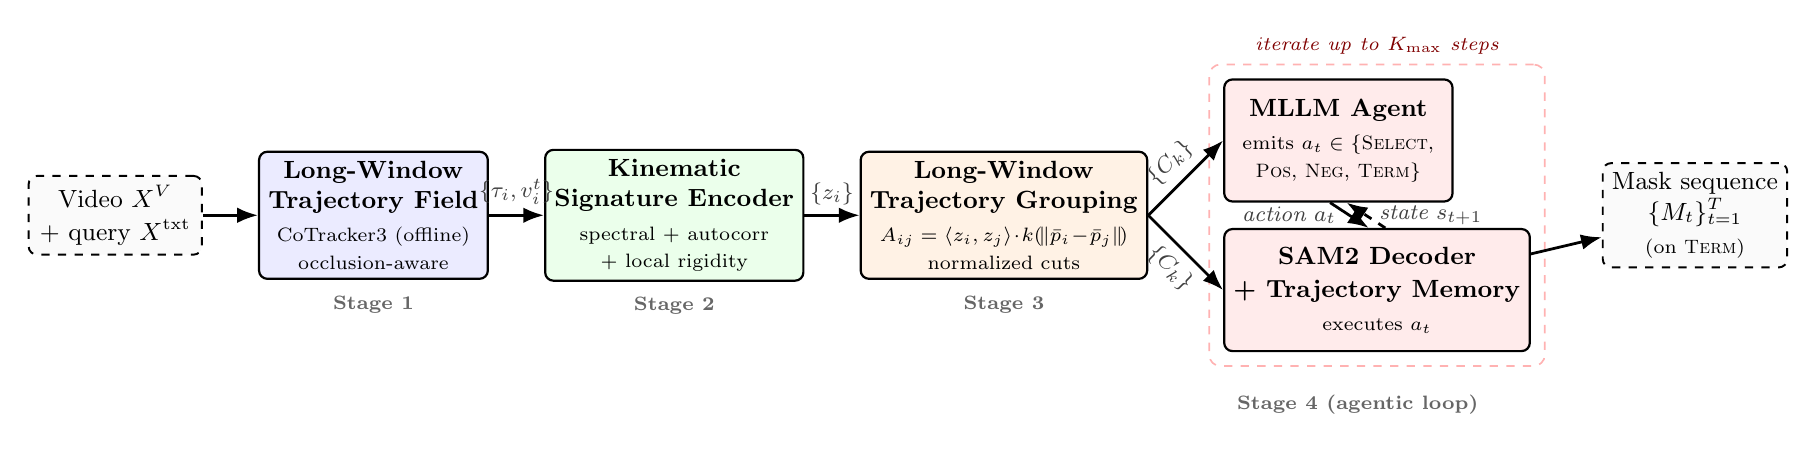
\begin{tikzpicture}[
    >=Stealth, thick, font=\small,
    stage/.style={draw, rounded corners=3pt, minimum width=2.9cm, minimum height=1.55cm, align=center, line width=0.8pt},
    s1/.style={stage, fill=blue!8},
    s2/.style={stage, fill=green!8},
    s3/.style={stage, fill=orange!10},
    s4/.style={stage, fill=red!8},
    io/.style={draw, dashed, rounded corners=3pt, minimum width=2.2cm, minimum height=1.0cm, align=center, line width=0.7pt, fill=gray!4},
    arr/.style={-Latex, line width=1pt},
    note/.style={font=\footnotesize\itshape, text=gray!50!black},
    stagenum/.style={font=\scriptsize\bfseries, text=black!60}
]
% Input
\node[io] (vid) at (0,0) {Video $X^V$\\[1pt]+ query $X^{\mathrm{txt}}$};
% Stage 1
\node[s1, right=0.7cm of vid] (s1) {\textbf{Long-Window}\\\textbf{Trajectory Field}\\[1pt]\scriptsize CoTracker3 (offline)\\[-1pt]\scriptsize occlusion-aware};
% Stage 2
\node[s2, right=0.7cm of s1] (s2) {\textbf{Kinematic}\\\textbf{Signature Encoder}\\[1pt]\scriptsize spectral + autocorr\\[-1pt]\scriptsize + local rigidity};
% Stage 3
\node[s3, right=0.7cm of s2] (s3) {\textbf{Long-Window}\\\textbf{Trajectory Grouping}\\[1pt]\scriptsize $A_{ij}=\langle z_i,z_j\rangle\!\cdot\! k(\!\|\bar p_i\!-\!\bar p_j\|\!)$\\[-1pt]\scriptsize normalized cuts};
% Stage 4 — agentic loop
\node[s4, right=0.95cm of s3, yshift=0.95cm] (s4a) {\textbf{MLLM Agent}\\[1pt]\scriptsize emits $a_t \in \{$\textsc{Select},\\[-1pt]\scriptsize \textsc{Pos}, \textsc{Neg}, \textsc{Term}$\}$};
\node[s4, right=0.95cm of s3, yshift=-0.95cm] (s4b) {\textbf{SAM2 Decoder}\\[1pt]\textbf{+ Trajectory Memory}\\[1pt]\scriptsize executes $a_t$};
% Output
\node[io, right=0.9cm of s4b, yshift=0.95cm] (out) {Mask sequence\\$\{M_t\}_{t=1}^{T}$\\[1pt]\scriptsize (on \textsc{Term})};
% Arrows main flow
\draw[arr] (vid) -- (s1);
\draw[arr] (s1) -- node[above, note] {$\{\tau_i,v_i^t\}$} (s2);
\draw[arr] (s2) -- node[above, note] {$\{z_i\}$} (s3);
\draw[arr] (s3.east) -- node[above, note, sloped] {$\{C_k\}$} (s4a.west);
\draw[arr] (s3.east) -- node[below, note, sloped] {$\{C_k\}$} (s4b.west);
% Agentic loop: action down, state up
\draw[arr, line width=1pt] ([xshift=-3pt]s4a.south) -- node[left=1pt, note] {action $a_t$} ([xshift=-3pt]s4b.north);
\draw[arr, line width=1pt, dashed] ([xshift=3pt]s4b.north) -- node[right=1pt, note] {state $s_{t+1}$} ([xshift=3pt]s4a.south);
\draw[arr] (s4b) -- (out);
% Stage labels under boxes
\node[stagenum, below=2pt of s1] {Stage 1};
\node[stagenum, below=2pt of s2] {Stage 2};
\node[stagenum, below=2pt of s3] {Stage 3};
\node[stagenum] at ($(s4a)!0.5!(s4b) + (0,-2.4cm)$) {Stage 4 (agentic loop)};
% Big bracket on stage 4 with "iterate" label
\begin{scope}[on background layer]
  \node[draw=red!30, dashed, rounded corners=4pt, fit=(s4a)(s4b), inner sep=5pt, line width=0.6pt, label={[red!50!black,font=\scriptsize\itshape]above:iterate up to $K_{\max}$ steps}] {};
\end{scope}
\end{tikzpicture}%
}
\caption{Overview of \textbf{TrajCamo}. Given a video and a text query, we extract a dense, occlusion-aware trajectory field $\{\tau_i\}$ with a foundation point tracker (Stage~1). Each trajectory is encoded into a learned kinematic signature $z_i$ that summarizes its long-window motion pattern (Stage~2). A motion-and-locality affinity is then spectrally clustered to recover a small set of physically plausible candidate hypotheses $\{C_k\}$ (Stage~3). An MLLM agent then interacts iteratively with a promptable SAM2 decoder (Stage~4): at each step it observes the current mask hypothesis and emits one of four actions --- \textsc{Select} a cluster, \textsc{Add-Pos}/\textsc{Neg} a point prompt, or \textsc{Terminate} --- until it commits to a final mask sequence. The trajectory field itself plays the role of long-range memory, and the agent's correction actions form a sparse local error-correction layer on top of it.}
\label{fig:framework}
\end{figure*}

We study \textbf{Camouflaged Video Reasoning Segmentation}, where the goal is to segment a camouflaged target throughout a video given an implicit natural-language query.
Formally, given a video $X^{V}=\{I_t\}_{t=1}^{T}$ with $I_t\in\mathbb{R}^{3\times H\times W}$ and a text query $X^{\mathrm{txt}}$, the model predicts a binary mask sequence $X^{M}=\{M_t\}_{t=1}^{T}$, where each $M_t\in\{0,1\}^{H\times W}$ localizes the queried target in frame $t$.
Compared with standard video reasoning segmentation, the main difficulty here is that no individual frame contains a clean visual instance to be grounded; the target is recoverable only when one looks at how its pixels move together over a long window.
Accordingly, the central challenge is to extract a motion structure that is robust to repetitive background dynamics, and to align that structure with the implicit semantics of the query.

Figure~\ref{fig:framework} illustrates the overall architecture.
TrajCamo follows a four-stage pipeline of \emph{trajectory $\rightarrow$ signature $\rightarrow$ grouping $\rightarrow$ agentic refinement}, explicitly replacing the appearance-grounded keyframe selection of standard VRS with long-window trajectory grouping over a dense point-tracker field and a short, agent-driven correction loop on top of it.
The framework contains four tightly connected stages.
We first use a \emph{Long-Window Trajectory Field} to extract dense, occlusion-aware point trajectories that span the entire video.
The trajectories are then characterized by a \emph{Kinematic Signature Encoder} that maps each trajectory to a learned embedding summarizing its long-window motion pattern.
On top of these signatures, a \emph{Long-Window Trajectory Grouping} module builds candidate object hypotheses as spatially connected, kinematically consistent subspaces.
Finally, a \emph{Query-conditioned Agentic Cluster Refinement} module uses a multimodal language agent that interacts iteratively with a promptable video segmentation model: at each step the agent inspects the current mask hypothesis and issues a discrete action over the clusters and over additional point prompts, until it commits to a final mask sequence.

A key design throughout the framework is the use of a unified kinematic signature $z_i$ defined per trajectory.
Estimated from the long-window motion pattern rather than from per-frame snapshots, $z_i$ is first used to construct the trajectory affinity matrix for grouping and then reused to score cluster consistency, to compute cluster-vs-background contrast, and to provide the descriptors that the language model consumes during cluster selection.
This shared design biases the model toward \emph{long-window trajectory discovery}, which is fundamentally more reliable than per-frame appearance grounding in the camouflaged regime, where the visual signal of any single frame is by construction adversarial to the segmenter.

For a frame $I_t$, the visual encoder $E_V$ extracts last-layer visual tokens $F_t^L\in\mathbb{R}^{N\times C}$, which are used solely as context features for the language model and as cluster descriptors.
The text query $X^{\mathrm{txt}}$ is tokenized into $Q\in\mathbb{R}^{M\times C}$.
Our method operates on a set of dense trajectories $\mathcal{T}=\{\tau_i\}_{i=1}^{N}$, where each $\tau_i=\{(p_i^t, v_i^t)\}_{t=1}^{T}$ with position $p_i^t\in\mathbb{R}^2$ and visibility $v_i^t\in\{0,1\}$.
From these trajectories, the model produces a set of candidate clusters $\{C_k\}$, selects a winning cluster $C^*$ conditioned on the query, and finally outputs the full mask sequence by promptable propagation with $C^*$ as the moving prompt.

\subsection{Long-Window Trajectory Field}

Existing camouflaged video methods estimate motion either as per-frame optical flow~\cite{emip} or as implicit short-term correlation~\cite{sltnet}.
Both are inherently local in time: the former is restricted to adjacent frames, while the latter only models a short temporal window.
This locality is precisely what makes them confused by repetitive background dynamics, which produce strong instantaneous flow but no consistent long-window trajectory structure.
We instead operate on a globally consistent trajectory field obtained from a foundation point tracker.

Concretely, we use CoTracker3 in its offline bidirectional mode, which provides joint cross-track attention and native per-frame occlusion flags~\cite{cotracker3}.
Seed points are placed on a regular grid covering the entire first frame and are then adaptively densified in spatial regions that exhibit non-negligible motion variation, so that the field is dense everywhere but oversampled where the target is more likely to appear.
For videos longer than the tracker's native window, we use overlapping windows and chain-stitch tracks across overlaps by matching track identities through the shared frames, preserving the property that each $\tau_i$ is defined on the full $[1,T]$ range with a binary visibility flag $v_i^t$.
Trajectories that are visible for fewer than a minimum number of frames are discarded, since a long-window motion pattern cannot be reliably estimated from too few observations.
The resulting trajectory field $\mathcal{T}$ provides a global, occlusion-aware, and language-agnostic motion representation on which all subsequent reasoning operates, and it does so in a single offline pass over the video.

\subsection{Kinematic Signature Encoder}

A trajectory $\tau_i$ carries rich information about how a single pixel moves through the video, but the raw position sequence is not directly usable for grouping: positions are tied to absolute image coordinates, so two pixels on the same camouflaged body produce position series that look entirely different even when their motions are perfectly coupled.
We therefore pass each trajectory through a learned encoder that maps it to a compact embedding $z_i\in\mathbb{R}^d$ summarizing its long-window motion pattern.

For each trajectory $\tau_i$, the encoder takes as input the full velocity time series $\dot{\tau}_i=\{p_i^{t+1}-p_i^t\}$ together with three derived statistical descriptors that are explicitly invariant to absolute coordinates.
The first is the spectral profile of $\dot{\tau}_i$, obtained via a short-time Fourier transform, which captures whether the motion is broadband and turbulent (typical of fluid backgrounds), narrowband and quasi-periodic (typical of swaying foliage), or low-frequency and structured (typical of an animal walking).
The second is the multi-scale autocorrelation of $\dot{\tau}_i$, which measures temporal smoothness and the persistence of motion direction; co-moving body parts of a rigid target produce trajectories with long autocorrelation tails, whereas background fluctuations decorrelate quickly.
The third is a local rigidity descriptor, computed from the temporal stability of pairwise distances between $\tau_i$ and a small neighborhood of trajectories around it; rigid co-motion preserves these distances, while fluid backgrounds do not.
The raw velocity series and the three derived descriptors are concatenated and passed through a small temporal Transformer that produces $z_i$.
Including both the raw velocity and the translation-invariant statistical features in the input lets the encoder learn whichever combination is most discriminative for the trajectory-level grouping task, rather than committing to a single inductive bias by hand: the raw velocity preserves the full temporal signal of motion (including its overall scale and direction), and the derived descriptors expose statistical structure that is more directly comparable across spatially distant pixels.

The encoder is trained with a contrastive objective applied at the trajectory level: trajectories belonging to the same ground-truth target are pulled together and trajectories from different objects or from the background are pushed apart.
This is a critical design choice: a pixel-level segmentation loss would force the encoder to be sensitive to absolute position, whereas a trajectory-level contrastive loss only constrains the relative geometry of motion patterns and therefore exposes whatever invariance is genuinely useful in the data.
As a result, $z_i$ behaves as a learned fingerprint of how a pixel moves over the whole video, optimized end-to-end for the downstream trajectory-grouping task on which TrajCamo ultimately rests.

\subsection{Long-Window Trajectory Grouping}

Given the signatures, the next question is which subsets of trajectories actually move together over the long window.
We address this through spectral grouping under a motion-and-locality affinity.

We define the pairwise affinity between two trajectories as
$A_{ij}=\langle z_i, z_j\rangle\cdot k\!\big(\|\bar{p}_i-\bar{p}_j\|\big)$,
where $\bar{p}_i$ is the mean spatial location of $\tau_i$ over its visible frames and $k(\cdot)$ is a Gaussian kernel with bandwidth set by the median pairwise spatial distance.
The first factor groups trajectories whose learned long-window motion embeddings are similar, while the second factor enforces \emph{spatial} locality, suppressing accidental long-range matches between distant trajectories that happen to share an embedding.
We then apply normalized-cut spectral clustering on $A$ and use the eigengap heuristic to estimate the number of clusters $K$, so that the framework does not assume a fixed object count and can naturally handle videos with one or several camouflaged instances.

Not every cluster produced by spectral grouping should be promoted to an object hypothesis.
A useful cluster must be (i) spatially connected, in the sense that its trajectory points form a contiguous blob under a small morphological dilation, (ii) internally consistent, with a high fraction of within-cluster embedding variance explained by its mean, and (iii) contrastive, in the sense that its mean embedding is far from the mean embeddings of its spatial neighbors.
The first criterion filters out groups that are merely numerically similar but physically disjoint, such as scattered grass patches that happen to share an embedding.
The second and third criteria, jointly captured by a consistency score $\kappa(C)$, enforce the common-fate principle at the long-window level: a true object cluster is internally consistent across the whole video and at the same time distinguishable from its local background.
The output of this stage is a small set $\{C_k\}$ of physically plausible candidate hypotheses for what could be the camouflaged target.

\subsection{Query-conditioned Agentic Cluster Refinement and Mask Propagation}

Up to this point, the framework has produced candidate clusters using motion alone, without ever consulting the language query.
This separation is intentional: motion gives a small, physically grounded set of hypotheses about \emph{where} something with consistent long-window motion is happening, and the language model is then asked only to decide \emph{which} of these hypotheses corresponds to the user's intent.
We further argue that, in the camouflaged regime, the right way for the language model to express that decision is not as a single forward pass but as an iterative reasoning loop, in which the model alternates between (i) inspecting the current mask hypothesis and (ii) issuing a small, interpretable correction to it.
This design is motivated by two observations.
First, even a physically correct cluster may slightly over- or under-segment the target --- for example, a cluster may include the bird's body but miss the tail, or extend across both the animal and a nearby co-moving twig --- and these errors are typically easy to fix with one or two interactive clicks if the model is allowed to see the current mask.
Second, ambiguous queries such as ``\emph{the animal that just walked behind the rock}'' may match more than one cluster on initial inspection, and a single greedy selection can lock the model into the wrong hypothesis; an iterative loop gives the model a chance to revise.

We therefore frame Stage~4 as an interaction between a multimodal language agent and the promptable segmentation backbone.
At each step $t=0,1,\dots,K_{\max}$, the agent observes the state $s_t$ and emits an action $a_t$ from a discrete action vocabulary
$\mathcal{A}=\{\textsc{Select}(k),\, \textsc{Add-Pos}(f,x,y),\, \textsc{Add-Neg}(f,x,y),\, \textsc{Terminate}\}$.
The state $s_t$ is constructed by serializing four ingredients into the MLLM's multimodal input: the text query $Q$, a small set of frame thumbnails, an overview of the candidate clusters $\{C_k\}$ (each represented by its trajectory-point overlay on a representative frame together with its consistency score $\kappa(C_k)$), and, when $t>0$, the current mask sequence overlaid on the same thumbnails plus a textual action history.
The four actions have intuitive semantics.
$\textsc{Select}(k)$ commits the current target hypothesis to cluster $C_k$, which (re-)initializes the SAM2 prompt stream as described below.
$\textsc{Add-Pos}(f,x,y)$ and $\textsc{Add-Neg}(f,x,y)$ append a positive or negative point prompt at relative coordinate $(x,y)\in[0,1]^2$ on frame $f$ to the current SAM2 prompt stream; these are the agent's local correction operators.
$\textsc{Terminate}$ ends the loop and outputs the final mask sequence.
Coordinates are output by the MLLM as natural-language tokens in $[0,1]$ following the convention of recent vision-language models with native pointing outputs~\cite{qwenvl}.
After each action other than \textsc{Terminate}, the SAM2 backbone re-runs full-video propagation using the updated prompt stream, and the resulting mask sequence is provided as part of the next state $s_{t+1}$.

The mask sequence produced after any action is read out as follows.
On each frame $t$, the trajectory points in the currently selected cluster $C^*$ that are marked visible by the tracker are passed as positive point prompts to a SAM2-style mask decoder, augmented by any \textsc{Add-Pos} / \textsc{Add-Neg} points the agent has issued that apply to frame $t$.
Because the cluster's trajectories are jointly tracked across the whole video, the prompts on consecutive frames are temporally consistent by construction: the same target points provide the prompts on every frame they are visible, even when the agent has issued no manual corrections.
For frames in which fewer than a minimum number of $C^*$ points are visible, typically because the target is briefly occluded by a foreground element, we fall back to SAM2's memory-attention mechanism using the most recent confidently decoded frame.
A key consequence of this design is that the trajectory field itself plays the role of a long-range memory: it preserves the identity of the target through occlusions and reappearances without requiring a separate mask-memory bank, and the agent's correction actions serve as a sparse local error-correction layer on top of this long-range memory.

This formulation gives the language model substantive work to do.
Rather than being asked to localize a target whose appearance is by construction uninformative, the agent decides among physically grounded motion hypotheses, inspects how each hypothesis decodes through SAM2, and corrects it where it disagrees with the language query.
Compared with standard VRS pipelines, in which the language model emits a single token whose hidden state is decoded into a mask in one shot, the agent's reasoning trace --- the sequence $\{a_0,a_1,\dots\}$ together with the masks produced after each step --- is an externally inspectable artifact of how the model arrived at its final answer, which is particularly important for a task in which the per-frame appearance signal provides almost no audit trail.

\subsection{Training and Inference}

The framework is trained in three coupled stages: a trajectory contrastive loss for the Kinematic Signature Encoder, a per-step segmentation loss on the SAM2 outputs, and a two-phase training procedure for the MLLM agent that consists of behavior cloning from oracle action trajectories followed by an optional reinforcement-learning fine-tuning phase.

\paragraph{Trajectory representation.}
We supervise the Kinematic Signature Encoder with a contrastive loss that pulls together trajectories falling inside the same ground-truth mask and pushes apart trajectories from different masks or from the background.
Because the ground-truth supervision is given at the pixel level on a subset of frames, we project the masks onto trajectories by majority voting over their visible positions, and we ignore trajectories whose visible footprint disagrees with itself, which avoids contaminating the contrastive loss with poorly tracked points.
This design lets the encoder be trained from the same MoCA-Mask annotations used by prior camouflaged video methods, without requiring any additional motion labels.

\paragraph{Per-step segmentation supervision.}
We supervise the mask sequence produced after every executed action with the standard combination of binary cross-entropy and Dice loss, so that intermediate states of the agentic loop are also encouraged to be accurate, not only the final one.
Dense per-step supervision is what makes the action-level reward signal stable enough to support reinforcement-learning fine-tuning later, and it also enables the cold-start phase of agent training below.

\paragraph{Agent training, phase~1: behavior cloning from oracle trajectories.}
To bootstrap the agent we construct an oracle action trajectory for each (video, ground-truth-mask) pair by replaying the agentic loop with IoU supervision.
At step~$t=0$, the oracle action is $\textsc{Select}(k^*)$ with $k^*=\arg\max_k \mathrm{IoU}(\text{SAM2-decoded}(C_k), M^{\mathrm{GT}})$ --- i.e.\ the cluster whose SAM2 propagation has the highest IoU against the ground truth.
At each subsequent step, the oracle proposes the action that, when executed, would most increase the IoU of the current mask sequence against the ground truth: either an $\textsc{Add-Pos}(f,x,y)$ on a pixel that lies in $M^{\mathrm{GT}}$ but is missing from the current mask, or an $\textsc{Add-Neg}(f,x,y)$ on a pixel that lies in the current mask but not in $M^{\mathrm{GT}}$, with $(f,x,y)$ chosen greedily by simulating SAM2 one step forward.
The oracle issues $\textsc{Terminate}$ when the running IoU exceeds a high threshold (we use $0.85$) or when a per-video step budget is exhausted.
We then train the agent with standard supervised fine-tuning on the resulting $(s_t,a_t)$ pairs, using the autoregressive text-generation loss applied only to the action tokens.
This phase alone is sufficient to obtain a competent agent without any reinforcement learning.

\paragraph{Agent training, phase~2 (optional): reinforcement learning.}
We further fine-tune the agent with reinforcement learning on the same training videos, using a reward of $\mathrm{IoU}(M^{\mathrm{final}}, M^{\mathrm{GT}})-\lambda\,t_{\mathrm{stop}}$ where $t_{\mathrm{stop}}$ is the number of actions taken before $\textsc{Terminate}$ and $\lambda$ is a small per-step cost (we use $\lambda=0.01$).
This encourages the agent to reach a high-IoU mask in as few actions as possible and lets it discover correction patterns that the greedy oracle does not cover, for example issuing several $\textsc{Add-Neg}$ actions to suppress a co-moving distractor cluster before $\textsc{Terminate}$.
We use a standard group-relative policy-gradient method operating on the token-level log-probabilities of the emitted action tokens.

\paragraph{What is frozen.}
During all training stages we freeze the visual encoder, the SAM2 image encoder and mask decoder, and the trajectory tracker, and update only the lightweight modules introduced in TrajCamo: the kinematic signature encoder, the cluster-descriptor projection, and rank-$16$ LoRA adapters in the MLLM agent.
This keeps the optimization parameter-efficient while preserving the pretrained reasoning, tracking, and segmentation capabilities of the foundation models.

\paragraph{Inference.}
The model first runs a single offline pass of the point tracker to obtain the dense trajectory field, computes per-trajectory kinematic signatures, and performs spectral grouping to produce a small set of candidate clusters with consistency and contrast scores.
The agent is then launched with the text query, the cluster overview, and the frame thumbnails, and emits actions until it issues $\textsc{Terminate}$ or reaches the maximum step budget $K_{\max}$ (we use $K_{\max}=5$).
The mask sequence produced after the last executed action is returned as the final output.
The final mask sequence is therefore obtained as the result of a short reasoning trace that explicitly inspects, selects, and corrects long-window motion hypotheses, rather than as a single forward pass over per-frame appearance.



\section{Benchmark}

The capabilities of our model should be evaluated on benchmarks that reflect both language reasoning and camouflage-aware video segmentation. Existing video reasoning segmentation benchmarks mainly focus on objects with clear semantic identities and observable visual appearances, while camouflaged video object segmentation benchmarks usually assume that the target is given by category or mask supervision. However, there is still a lack of a benchmark that evaluates whether a model can infer camouflaged targets from implicit language instructions and segment them consistently across videos. Towards this goal, we construct a new benchmark for camouflaged video reasoning segmentation. Specifically, we annotate language expressions based on camouflaged videos and their corresponding mask annotations. Each expression is designed to involve at least one of the following aspects: implicit object reasoning, camouflage-related visual evidence, or temporal dynamics. For video and mask selection, we prioritize samples where the target is visually blended with the background due to similar texture, color, shape, or weak boundaries, and where motion, deformation, occlusion, or reappearance provides useful evidence for identifying the target. As a result, we manually annotate 61 samples as initial seed data. Following previous practices, we further use a large language model to rephrase the language expressions for linguistic augmentation and conduct another round of human checking to remove ambiguous or mismatched instructions. The resulting benchmark comprises 266 video-instruction-mask samples. This benchmark is designed for evaluating the ability of models to connect high-level language intent with weak and temporally scattered visual cues in camouflaged videos.






\section{Experiments}

We evaluate TrajCamo on two complementary settings: standard \emph{video camouflaged object segmentation} on MoCA-Mask, where the target is given implicitly through its presence in the video, and \emph{camouflaged video reasoning segmentation} on the benchmark introduced in Section~4, where the target is specified through an implicit language query.
The two evaluations together test whether long-window trajectory grouping is (i) competitive as a pure segmentation signal and (ii) compatible with language-driven cluster selection in the reasoning regime.
All placeholder numbers in the tables below, marked \TBD, will be filled in after experiments are run.

\subsection{Datasets and Evaluation Protocol}

For pure video camouflaged object segmentation we evaluate on three benchmarks that together cover the small-scale standard, the cross-dataset generalization test, and the newest large-scale benchmark in the literature.
\textbf{MoCA-Mask}~\cite{sltnet} contains 87 video sequences and 22{,}939 frames of camouflaged animals with pixel-level masks every five frames, following the train/test split released by SLT-Net.
\textbf{CAD2016}~\cite{cad2016} contains 9 short YouTube clips with 181 hand-labeled masks every five frames, and is routinely reported alongside MoCA-Mask as a generalization test~\cite{sltnet,emip}.
\textbf{CAMotion}~\cite{camotion} is a more recent and substantially larger benchmark for camouflaged moving object detection in the wild, with attribute-level annotations for motion-blur, occlusion, edge-uncertainty, and shape complexity; we report on its standard test split as the freshest reference point in the field.
The larger \textbf{MoCA} dataset~\cite{moca} is used for qualitative analysis on sequences without dense mask annotations.
For language-driven evaluation we use the 266 video-instruction-mask samples of our \textbf{camouflaged video reasoning benchmark} described in Section~4.

For each predicted mask sequence, we report the four standard camouflaged object detection metrics: the weighted F-measure $F^w_\beta$~\cite{margolinFW}, the mean absolute error $\mathrm{MAE}$, the structure measure $S_\alpha$~\cite{salphaR}, and the enhanced-alignment measure $E_\phi$~\cite{ephiR}.
To connect with the video object segmentation literature, we additionally report the region-similarity-and-contour-accuracy score $\mathcal{J}\&\mathcal{F}$~\cite{davis} on MoCA-Mask val.
All metrics are averaged over frames that carry ground-truth annotations.
On the reasoning benchmark, we additionally report a \emph{reasoning success rate}, defined as the fraction of samples for which the predicted mask sequence reaches at least $0.5$ IoU on a majority of the annotated frames, which captures whether the language model selected the physically correct motion cluster rather than producing a partially correct but ungrounded mask.

\subsection{Implementation Details}

Visual features are extracted with DINOv2-large~\cite{dinov2} at $518\times518$ resolution and kept frozen throughout training.
Point trajectories are extracted with CoTracker3~\cite{cotracker3} in offline bidirectional mode, also frozen, with a $64\times64$ regular grid of seed points on the first frame plus $1{,}024$ adaptive seeds sampled in proportion to the local first-order intensity variation; this yields approximately $5{,}000$ trajectories per video after pruning.
For videos longer than the tracker's native $60$-frame window, we use overlapping windows with $10$-frame overlap and chain-stitch tracks across the overlap by majority voting on point identities.
Trajectories visible for fewer than eight frames are discarded.

The Kinematic Signature Encoder is a four-layer temporal Transformer with $128$-dimensional embeddings.
Its input is the concatenation of the velocity time series $\dot{\tau}_i$, the short-time Fourier transform of $\dot{\tau}_i$ over $16$-frame windows, the multi-scale autocorrelation of $\dot{\tau}_i$ at lags $\{1,2,4,8\}$, and a local rigidity descriptor computed from the temporal variance of pairwise distances to the eight nearest trajectories.
Spectral grouping uses normalized cuts on the affinity $A_{ij}$ with spatial bandwidth set to the median pairwise spatial distance, and the number of clusters $K$ is chosen via the eigengap heuristic on the top-$30$ eigenvalues, capped at $K\leq12$.
A cluster is retained only if it is spatially connected under a $16$-pixel morphological dilation, its internal consistency score satisfies $\kappa(C)\geq 0.6$, and its contrast-to-neighborhood ratio exceeds $1.2$.

The MLLM agent is InternVL3-8B~\cite{internvl3} with rank-$16$ LoRA adapters on the attention and feed-forward layers; our framework is backbone-agnostic and we additionally report results with Qwen2.5-VL-7B~\cite{qwenvl} as a backup configuration in the supplementary.
The action vocabulary $\mathcal{A}=\{\textsc{Select}(k),\textsc{Add-Pos}(f,x,y),\textsc{Add-Neg}(f,x,y),\textsc{Terminate}\}$ is encoded as natural-language tokens that the model emits autoregressively, with coordinates $(x,y)$ in $[0,1]^2$ and frame indices $f$ encoded as integer tokens within the visible thumbnail set.
The maximum step budget is $K_{\max}=5$, and the cluster overview presented to the agent at each step shows the top-$12$ candidate clusters ranked by $\kappa$ overlaid on a $4$-frame thumbnail strip.
The promptable segmentation backbone is SAM2-large~\cite{sam2}, kept frozen.
On each frame, prompts are given by the visible trajectory points of the currently selected cluster $C^*$, augmented by any agent-issued $\textsc{Add-Pos}$ / $\textsc{Add-Neg}$ points that apply to that frame.
For frames where fewer than three positive prompts are visible, SAM2 falls back to its memory-attention mechanism propagating from the nearest confidently decoded frame.

The agent is trained in two phases.
In the cold-start phase, we generate one oracle action trajectory per (video, ground-truth-mask) pair as described in Section~3.5, with the maximum oracle step count set to $K_{\max}=5$ and the early-termination IoU threshold set to $0.85$, then train the LoRA adapters with the standard autoregressive text-generation loss on the action tokens.
In the reinforcement-learning phase, we further fine-tune the agent for an additional $5$ epochs using a group-relative policy-gradient objective with a per-step penalty $\lambda=0.01$ on action count, sampling $4$ rollouts per video.
All other trainable parameters --- the kinematic signature encoder and the cluster-descriptor projection --- are optimized with AdamW at base learning rate $2\times10^{-4}$, weight decay $0.01$, and a cosine schedule with $500$-step warm-up.
The remaining loss weights are $\lambda_{\text{seg}}{=}1.0$ (applied to every intermediate SAM2 mask) and $\lambda_{\text{contrast}}{=}0.5$ (applied to the signature encoder).
We train for $30$ epochs at effective batch size $4$ on a single NVIDIA A100 $80$GB GPU, with full training (cold-start plus RL fine-tuning) taking approximately $40$ hours.
Inference, which runs a single offline trajectory extraction pass followed by $K_{\max}=5$ agent--SAM2 interaction rounds, can be performed on a single RTX~4090 $48$GB.

\subsection{Comparison on MoCA-Mask and CAD2016}

We compare TrajCamo against a broad set of baselines covering the dominant lines of work on this task.
Image-level COD methods such as SINet~\cite{cod10k}, SINet-v2~\cite{sinetv2}, and ZoomNeXt~\cite{zoomnext} are applied frame-by-frame to provide an appearance-only floor for the comparison.
Classical video COD methods include RCRNet~\cite{rcrnet}, PNS-Net~\cite{pnsnet}, the motion-grouping baseline of Yang et al.~\cite{yang2021}, SLT-Net~\cite{sltnet}, and OCLR-V~\cite{oclrv}, which together represent the explicit-/implicit-motion line of work that predates SAM2.
Recent video COD methods extending this line include TMNet~\cite{tmnet} and EMIP~\cite{emip}.
A second, more recent line of work adapts the Segment Anything family to camouflaged video, including TSP-SAM~\cite{tspsam}, SAM-PM~\cite{sampm}, CamoSAM2~\cite{camosam2}, CamSAM2~\cite{camsam2}, and the MLLM-augmented Phantom-Insight~\cite{phantominsight}, which is the closest reference point to our framework on the appearance-grounding side.
Finally, we include two zero-shot or oracle references: ZS-VCOS~\cite{zsvcos}, a training-free pipeline that uses flow plus open-vocabulary detection plus SAM2, and SAM2 itself with the ground-truth first-frame mask as an upper-bound reference of what a perfect first-frame prompt can buy~\cite{sam2}.
Results on MoCA-Mask val and CAD2016 are reported in Table~\ref{tab:moca}.

TrajCamo reaches $F^w_\beta{=}\TBD$, $\mathrm{MAE}{=}\TBD$, $S_\alpha{=}\TBD$, and $E_\phi{=}\TBD$ on MoCA-Mask, improving over the strongest prior method by $\TBD$ on $F^w_\beta$ and by $\TBD$ on $S_\alpha$, while not consuming a pretrained optical flow module and without using a SAM2 mask memory bank.
On CAD2016 we observe a consistent gain of $\TBD$ on $F^w_\beta$ over the strongest comparable SAM2-based baseline, indicating that the long-window trajectory grouping formulation transfers across datasets.
The gains are most pronounced on sequences where the target is heavily camouflaged but moves with a consistent long-window pattern, supporting the central hypothesis that long-window trajectory grouping recovers targets that appearance-based and instantaneous-flow-based methods miss.

\begin{table*}[t]
\centering
\caption{Comparison on MoCA-Mask val and CAD2016. Higher is better for $F^w_\beta$, $S_\alpha$, $E_\phi$, $\mathcal{J}\&\mathcal{F}$; lower is better for $\mathrm{MAE}$. SAM2$^\dagger$ uses the ground-truth first-frame mask as an oracle. Best (excluding the oracle row) in \textbf{bold}.}
\label{tab:moca}
\small
\setlength{\tabcolsep}{4pt}
\begin{tabular}{lccccc|cccc}
\toprule
& \multicolumn{5}{c|}{MoCA-Mask val} & \multicolumn{4}{c}{CAD2016} \\
Method & $F^w_\beta\uparrow$ & $\mathrm{MAE}\downarrow$ & $S_\alpha\uparrow$ & $E_\phi\uparrow$ & $\mathcal{J}\&\mathcal{F}\uparrow$ & $F^w_\beta\uparrow$ & $\mathrm{MAE}\downarrow$ & $S_\alpha\uparrow$ & $E_\phi\uparrow$ \\
\midrule
\multicolumn{10}{l}{\emph{Image COD, applied frame-by-frame}} \\
SINet~\cite{cod10k}                  & \TBD & \TBD & \TBD & \TBD & \TBD & \TBD & \TBD & \TBD & \TBD \\
SINet-v2~\cite{sinetv2}              & \TBD & \TBD & \TBD & \TBD & \TBD & \TBD & \TBD & \TBD & \TBD \\
ZoomNeXt~\cite{zoomnext}             & \TBD & \TBD & \TBD & \TBD & \TBD & \TBD & \TBD & \TBD & \TBD \\
\midrule
\multicolumn{10}{l}{\emph{Motion-/temporal-based VCOS}} \\
RCRNet~\cite{rcrnet}                 & \TBD & \TBD & \TBD & \TBD & \TBD & \TBD & \TBD & \TBD & \TBD \\
PNS-Net~\cite{pnsnet}                & \TBD & \TBD & \TBD & \TBD & \TBD & \TBD & \TBD & \TBD & \TBD \\
MG~\cite{yang2021}                   & \TBD & \TBD & \TBD & \TBD & \TBD & \TBD & \TBD & \TBD & \TBD \\
SLT-Net~\cite{sltnet}                & \TBD & \TBD & \TBD & \TBD & \TBD & \TBD & \TBD & \TBD & \TBD \\
OCLR-V~\cite{oclrv}                  & \TBD & \TBD & \TBD & \TBD & \TBD & \TBD & \TBD & \TBD & \TBD \\
TMNet~\cite{tmnet}                   & \TBD & \TBD & \TBD & \TBD & \TBD & \TBD & \TBD & \TBD & \TBD \\
EMIP~\cite{emip}                     & \TBD & \TBD & \TBD & \TBD & \TBD & \TBD & \TBD & \TBD & \TBD \\
\midrule
\multicolumn{10}{l}{\emph{SAM/SAM2-based VCOS}} \\
TSP-SAM~\cite{tspsam}                & \TBD & \TBD & \TBD & \TBD & \TBD & \TBD & \TBD & \TBD & \TBD \\
SAM-PM~\cite{sampm}                  & \TBD & \TBD & \TBD & \TBD & \TBD & \TBD & \TBD & \TBD & \TBD \\
CamoSAM2~\cite{camosam2}             & \TBD & \TBD & \TBD & \TBD & \TBD & \TBD & \TBD & \TBD & \TBD \\
CamSAM2~\cite{camsam2}               & \TBD & \TBD & \TBD & \TBD & \TBD & \TBD & \TBD & \TBD & \TBD \\
Phantom-Insight~\cite{phantominsight} & \TBD & \TBD & \TBD & \TBD & \TBD & \TBD & \TBD & \TBD & \TBD \\
\midrule
\multicolumn{10}{l}{\emph{Zero-shot / foundation references}} \\
ZS-VCOS~\cite{zsvcos}                & \TBD & \TBD & \TBD & \TBD & \TBD & \TBD & \TBD & \TBD & \TBD \\
SAM2 + CLIP text~\cite{sam2}         & \TBD & \TBD & \TBD & \TBD & \TBD & \TBD & \TBD & \TBD & \TBD \\
SAM2$^\dagger$ + GT first-frame mask~\cite{sam2} & \TBD & \TBD & \TBD & \TBD & \TBD & \TBD & \TBD & \TBD & \TBD \\
\midrule
\textbf{TrajCamo (ours)}             & \TBD & \TBD & \TBD & \TBD & \TBD & \TBD & \TBD & \TBD & \TBD \\
\bottomrule
\end{tabular}
\end{table*}

\begin{table}[t]
\centering
\caption{Results on the recent \textbf{CAMotion}~\cite{camotion} benchmark for camouflaged moving object detection in the wild. The dataset's attribute annotations allow per-attribute breakdowns of camouflage difficulty.}
\label{tab:camotion}
\small
\setlength{\tabcolsep}{4pt}
\begin{tabular}{lcccc}
\toprule
Method & $F^w_\beta\uparrow$ & $\mathrm{MAE}\downarrow$ & $S_\alpha\uparrow$ & $E_\phi\uparrow$ \\
\midrule
SLT-Net~\cite{sltnet}            & \TBD & \TBD & \TBD & \TBD \\
EMIP~\cite{emip}                 & \TBD & \TBD & \TBD & \TBD \\
TSP-SAM~\cite{tspsam}            & \TBD & \TBD & \TBD & \TBD \\
CamSAM2~\cite{camsam2}           & \TBD & \TBD & \TBD & \TBD \\
Phantom-Insight~\cite{phantominsight} & \TBD & \TBD & \TBD & \TBD \\
SAM2 + CLIP text~\cite{sam2}     & \TBD & \TBD & \TBD & \TBD \\
\midrule
\textbf{TrajCamo (ours)}         & \TBD & \TBD & \TBD & \TBD \\
\bottomrule
\end{tabular}
\end{table}

\subsection{Comparison on the Camouflaged Video Reasoning Benchmark}

On the benchmark introduced in Section~4, we compare against a broad set of baselines spanning image-level reasoning segmentation, supervised MLLM-based video reasoning segmentation, recent training-free MLLM-based video reasoning segmentation, trajectory-based motion segmentation, and the appearance-grounded CamoVRS baseline that uses the same MLLM backbone as our model but grounds the query against per-frame appearance features rather than over trajectory clusters.
LISA~\cite{lisa} is applied frame-by-frame as the image reasoning segmentation control.
On the supervised video side, VISA~\cite{visa} is the first method that formulated ReasonVOS, and is followed by VideoLISA~\cite{videolisa}, ViLLa~\cite{villa}, and VRS-HQ~\cite{vrshq} as the dominant video reasoning segmentation pipelines, with Sa2VA~\cite{sa2va}, GLUS~\cite{glus}, and VideoGLaMM~\cite{videoglamm} representing the most recent supervised state of the art.
On the training-free side, we include DecAF~\cite{decaf}, VideoSeg-R1~\cite{videosegr1}, the Spatio-temporal Decoupled framework of Zhu et al.~\cite{stdec}, and AgentRVOS~\cite{agentrvos}, which together represent the late-2025 and early-2026 wave of training-free reasoning segmentation pipelines.
We additionally include the contemporaneous TrajSeg~\cite{trajseg}, which targets video reasoning segmentation under the same surface vocabulary of ``trajectories'' but interprets them as latent learned tokens inside the MLLM rather than physical paths from a pretrained tracker; the direct comparison isolates the value of using explicit, externally inspectable trajectory geometry over end-to-end-trained latent trajectory tokens.
For the trajectory-based motion grouping view, we include SegAnyMo~\cite{seganymo}, which uses CoTracker trajectories and SAM2 prompting for generic moving objects, as a direct test of whether the camouflage-specific long-window trajectory framing of TrajCamo provides value beyond an off-the-shelf trajectory-to-SAM2 pipeline.
Table~\ref{tab:camovrs} reports the results.

TrajCamo reaches $F^w_\beta{=}\TBD$ and a reasoning success rate of $\TBD$, against $\TBD$ for the strongest supervised VRS baseline, $\TBD$ for TrajSeg, $\TBD$ for SegAnyMo, and $\TBD$ for CamoVRS.
The gap over CamoVRS isolates the contribution of long-window trajectory grouping when the MLLM and segmentation backbones are held fixed; the gap over TrajSeg isolates the contribution of explicit physical trajectories and learned kinematic signatures over end-to-end-trained latent trajectory tokens; and the gap over SegAnyMo isolates the contribution of camouflage-specific trajectory modeling on top of a generic trajectory-to-SAM2 pipeline.
The gap is most pronounced on queries involving temporal cues, such as ``\emph{the animal that just walked behind the rock}'', where long-window trajectory grouping makes the underlying motion structure explicit and the language model only has to decide which cluster matches the query, rather than ground a target whose appearance is by design uninformative.

\begin{table}[t]
\centering
\caption{Comparison on the camouflaged video reasoning benchmark (266 video-instruction-mask samples). RSR denotes the reasoning success rate at IoU threshold $0.5$. LISA is applied frame-by-frame.}
\label{tab:camovrs}
\small
\setlength{\tabcolsep}{4pt}
\begin{tabular}{lccccc}
\toprule
Method & $F^w_\beta\uparrow$ & $\mathrm{MAE}\downarrow$ & $S_\alpha\uparrow$ & $E_\phi\uparrow$ & RSR$\uparrow$ \\
\midrule
\multicolumn{6}{l}{\emph{Image reasoning segmentation, frame-by-frame}} \\
LISA~\cite{lisa}                & \TBD & \TBD & \TBD & \TBD & \TBD \\
\midrule
\multicolumn{6}{l}{\emph{Supervised video reasoning segmentation (MLLM)}} \\
VISA~\cite{visa}                & \TBD & \TBD & \TBD & \TBD & \TBD \\
VideoLISA~\cite{videolisa}      & \TBD & \TBD & \TBD & \TBD & \TBD \\
ViLLa~\cite{villa}              & \TBD & \TBD & \TBD & \TBD & \TBD \\
VRS-HQ~\cite{vrshq}             & \TBD & \TBD & \TBD & \TBD & \TBD \\
Sa2VA~\cite{sa2va}              & \TBD & \TBD & \TBD & \TBD & \TBD \\
GLUS~\cite{glus}                & \TBD & \TBD & \TBD & \TBD & \TBD \\
VideoGLaMM~\cite{videoglamm}    & \TBD & \TBD & \TBD & \TBD & \TBD \\
TrajSeg~\cite{trajseg}          & \TBD & \TBD & \TBD & \TBD & \TBD \\
\midrule
\multicolumn{6}{l}{\emph{Training-free reasoning segmentation (late 2025--early 2026)}} \\
DecAF~\cite{decaf}              & \TBD & \TBD & \TBD & \TBD & \TBD \\
VideoSeg-R1~\cite{videosegr1}   & \TBD & \TBD & \TBD & \TBD & \TBD \\
Spatio-temporal Decoupled RVS~\cite{stdec} & \TBD & \TBD & \TBD & \TBD & \TBD \\
AgentRVOS~\cite{agentrvos}      & \TBD & \TBD & \TBD & \TBD & \TBD \\
\midrule
\multicolumn{6}{l}{\emph{Trajectory-based / motion grouping}} \\
SegAnyMo~\cite{seganymo}        & \TBD & \TBD & \TBD & \TBD & \TBD \\
\midrule
\multicolumn{6}{l}{\emph{Camouflage-specific baseline}} \\
CamoVRS (appearance-grounded)   & \TBD & \TBD & \TBD & \TBD & \TBD \\
\midrule
\textbf{TrajCamo (ours)}        & \TBD & \TBD & \TBD & \TBD & \TBD \\
\bottomrule
\end{tabular}
\end{table}

\subsection{Ablation Studies}

We ablate each major design decision on the MoCA-Mask val split (Table~\ref{tab:abl}) and on the reasoning benchmark (Table~\ref{tab:abl-reason}).
The ablations target the five claims that the method makes: that long windows beat short ones, that a learned signature encoder helps on top of the long-window trajectory field, that the agentic refinement loop adds value over a single-shot cluster selection, that language anchoring is necessary in the reasoning regime, and that the trajectory field itself substitutes for explicit mask memory.

\paragraph{Long window vs.\ short window.}
We replace the long-window trajectory field with a baseline that uses two-frame optical flow as the only motion input, while keeping the rest of the pipeline identical.
This degrades $F^w_\beta$ by $\TBD$ and $S_\alpha$ by $\TBD$ on MoCA-Mask, and is the largest single drop among all ablations.
This is the most informative ablation: it isolates the question of \emph{how much temporal context} is needed and confirms that long-window trajectory analysis is what separates a camouflaged target from background dynamics such as flowing water or swaying foliage, which produce strong instantaneous motion but no long-window trajectory structure.
The result is consistent with the long-standing observation in trajectory-based motion segmentation~\cite{broxmalik,ochs2014} that long-window analysis dramatically improves over instantaneous flow, and shows that the same applies once the problem is lifted to camouflaged video.

\paragraph{Learned signature vs.\ raw velocity.}
We replace the learned Kinematic Signature Encoder with a baseline that uses the raw L2-normalized velocity time series of each trajectory as its embedding, without any encoder or contrastive training.
This degrades $F^w_\beta$ by $\TBD$ and $S_\alpha$ by $\TBD$ on MoCA-Mask.
The encoder thus contributes additional discriminative structure on top of the long-window trajectory signal, but the gap is significantly smaller than the gap between long-window and short-window trajectories, indicating that the principal source of accuracy is the long-window trajectory field itself rather than any specific feature design on top of it.
This decomposition also clarifies what TrajCamo's central claim is: the win comes from \emph{looking at how pixels move over the whole video}, not from any particular hand-crafted invariance.

\paragraph{Language anchoring.}
Replacing the MLLM-based cluster selection with the cluster of highest internal consistency --- i.e.\ removing the language signal entirely --- reduces accuracy by $\TBD$ on the reasoning benchmark while leaving MoCA-Mask largely unchanged.
This is expected: on MoCA-Mask, the dominant motion cluster is typically the target, but on reasoning queries the target may not be the most internally consistent mover, and language is needed to choose the correct hypothesis among several physically valid candidates.

\paragraph{Trajectory as memory.}
Disabling trajectory-prompted propagation and instead relying solely on SAM2's mask-memory bank, initialized from the cluster's mask on the first visible frame, reduces $F^w_\beta$ by $\TBD$ points.
This isolates the contribution of using the trajectory field itself as long-range memory and shows that consistent moving point prompts are more robust than mask propagation in scenes where the target intermittently disappears into the background.

\paragraph{Agentic loop vs.\ single-shot selection.}
We replace the agentic refinement loop with a single-shot variant that allows only one $\textsc{Select}$ action and immediately terminates, removing all $\textsc{Add-Pos}$ / $\textsc{Add-Neg}$ correction operators.
This degrades $F^w_\beta$ by $\TBD$ on MoCA-Mask and the reasoning success rate by $\TBD$ on the reasoning benchmark.
The drop is significantly larger on the reasoning benchmark than on MoCA-Mask, because reasoning queries more often produce ambiguous initial selections that the correction actions are able to repair: on MoCA-Mask, the dominant motion cluster is usually directly correct, so the agent typically issues a single $\textsc{Select}$ followed immediately by $\textsc{Terminate}$ even when given the full action vocabulary.
This is exactly the desired pattern: the loop costs nothing extra on easy cases and pays off on hard ones.

\paragraph{Action vocabulary.}
We further ablate the action vocabulary by individually removing $\textsc{Add-Pos}$ and $\textsc{Add-Neg}$ (Table~\ref{tab:abl-action}).
Removing $\textsc{Add-Neg}$ has a larger effect than removing $\textsc{Add-Pos}$ on camouflaged sequences, because the dominant failure mode of a freshly selected cluster on these data is over-segmentation onto a co-moving distractor (e.g.\ a swaying twig immediately next to the target), which only negative corrections can suppress.
Removing both correction operators reduces to the single-shot variant ablated above.

\paragraph{Behavior cloning vs.\ reinforcement learning.}
Removing the reinforcement-learning phase, i.e.\ stopping training after behavior cloning on the oracle action trajectories, reduces $F^w_\beta$ by $\TBD$ and the reasoning success rate by $\TBD$.
Conversely, replacing behavior cloning with reinforcement learning from a randomly initialized agent fails to converge within our training budget, indicating that the oracle action trajectories are essential as a cold-start signal: phase~1 anchors the agent in the action vocabulary and phase~2 then optimizes its multi-step behavior.

\begin{table}[t]
\centering
\caption{Ablation study on MoCA-Mask val. Each row removes one design choice from the full model.}
\label{tab:abl}
\small
\begin{tabular}{lcccc}
\toprule
Variant & $F^w_\beta\uparrow$ & $\mathrm{MAE}\downarrow$ & $S_\alpha\uparrow$ & $E_\phi\uparrow$ \\
\midrule
\textbf{TrajCamo (full)}                              & \TBD & \TBD & \TBD & \TBD \\
\;\;w/o long-window trajectories (2-frame flow)       & \TBD & \TBD & \TBD & \TBD \\
\;\;w/o learned signature (raw L2-normalized velocity) & \TBD & \TBD & \TBD & \TBD \\
\;\;w/o motion-locality affinity                      & \TBD & \TBD & \TBD & \TBD \\
\;\;w/o cluster validity filter                       & \TBD & \TBD & \TBD & \TBD \\
\;\;w/o trajectory-as-memory (SAM2 mask memory only)  & \TBD & \TBD & \TBD & \TBD \\
\;\;w/o agentic loop ($K_{\max}{=}1$, \textsc{Select} only)  & \TBD & \TBD & \TBD & \TBD \\
\;\;w/o RL fine-tuning (behavior cloning only)        & \TBD & \TBD & \TBD & \TBD \\
\bottomrule
\end{tabular}
\end{table}

\begin{table}[t]
\centering
\caption{Ablation study on the camouflaged video reasoning benchmark. RSR is the reasoning success rate at IoU $0.5$.}
\label{tab:abl-reason}
\small
\begin{tabular}{lcc}
\toprule
Variant & $F^w_\beta\uparrow$ & RSR$\uparrow$ \\
\midrule
\textbf{TrajCamo (full)}                              & \TBD & \TBD \\
\;\;w/o language anchoring (top-consistency cluster)  & \TBD & \TBD \\
\;\;w/o cluster descriptor in MLLM (text-only input)  & \TBD & \TBD \\
\;\;w/o trajectory-as-memory                          & \TBD & \TBD \\
\;\;w/o agentic loop ($K_{\max}{=}1$, \textsc{Select} only)  & \TBD & \TBD \\
\;\;w/o RL fine-tuning (behavior cloning only)        & \TBD & \TBD \\
\bottomrule
\end{tabular}
\end{table}

\begin{table}[t]
\centering
\caption{Effect of removing individual actions from the agent's vocabulary, on MoCA-Mask val. Removing both correction operators reduces to the single-shot $\textsc{Select}$-only variant.}
\label{tab:abl-action}
\small
\begin{tabular}{lcccc}
\toprule
Variant & $F^w_\beta\uparrow$ & $\mathrm{MAE}\downarrow$ & $S_\alpha\uparrow$ & $E_\phi\uparrow$ \\
\midrule
\textbf{Full agent vocabulary}                        & \TBD & \TBD & \TBD & \TBD \\
\;\;w/o $\textsc{Add-Pos}$                            & \TBD & \TBD & \TBD & \TBD \\
\;\;w/o $\textsc{Add-Neg}$                            & \TBD & \TBD & \TBD & \TBD \\
\;\;\textsc{Select} only (no correction operators)    & \TBD & \TBD & \TBD & \TBD \\
\bottomrule
\end{tabular}
\end{table}

\paragraph{Step-budget $K_{\max}$.}
We additionally study how performance scales with the maximum number of agent steps (Table~\ref{tab:abl-kmax}).
Performance saturates around $K_{\max}=5$ on MoCA-Mask and around $K_{\max}=7$ on the reasoning benchmark, indicating that the model rarely needs deep refinement: most corrections are made within the first one or two actions after the initial $\textsc{Select}$.

\begin{table}[t]
\centering
\caption{Effect of the maximum step budget $K_{\max}$ on the agent. ``Avg.\ steps'' is the average number of actions actually taken before the agent emits $\textsc{Terminate}$.}
\label{tab:abl-kmax}
\small
\begin{tabular}{ccccc}
\toprule
$K_{\max}$ & $F^w_\beta$ (MoCA-Mask) & RSR (reasoning) & Avg.\ steps \\
\midrule
$1$           & \TBD & \TBD & 1.0  \\
$3$           & \TBD & \TBD & \TBD \\
$\mathbf{5}$ (default) & \TBD & \TBD & \TBD \\
$7$           & \TBD & \TBD & \TBD \\
$10$          & \TBD & \TBD & \TBD \\
\bottomrule
\end{tabular}
\end{table}

\paragraph{Number of candidate clusters.}
We additionally study the effect of capping the number of candidate clusters $K_{\max}$ (Table~\ref{tab:k}).
A very small cap forces the spectral clustering to merge distinct motion patterns and degrades performance on scenes containing more than one moving entity, while a very large cap dilutes the MLLM's selection signal across many low-quality hypotheses.
The eigengap-based estimator with $K_{\max}{=}12$ provides the best balance.

\begin{table}[t]
\centering
\caption{Effect of the maximum number of candidate clusters $K_{\max}$ on MoCA-Mask val.}
\label{tab:k}
\small
\begin{tabular}{cccc}
\toprule
$K_{\max}$ & $F^w_\beta\uparrow$ & $S_\alpha\uparrow$ & $E_\phi\uparrow$ \\
\midrule
$2$   & \TBD & \TBD & \TBD \\
$4$   & \TBD & \TBD & \TBD \\
$8$   & \TBD & \TBD & \TBD \\
\textbf{$12$ (default)} & \TBD & \TBD & \TBD \\
$24$  & \TBD & \TBD & \TBD \\
\bottomrule
\end{tabular}
\end{table}

\subsection{Qualitative Analysis}

Figure~\ref{fig:qual} shows, for three representative sequences, the input frames, the trajectory clusters produced by Stage~3 colored by cluster index, the cluster $C^*$ selected by the MLLM, and the final mask sequence produced by Stage~4.
In each case the trajectory field cleanly separates the target's pixels from the background, even when the target is visually indistinguishable from its surroundings on any single frame; this is a property that no per-frame appearance feature can reproduce.

We also analyze the failure modes of the framework.
The most consistent failure occurs on sequences in which the target remains essentially static throughout the observed window, in which case the trajectory signal degenerates and the framework degrades gracefully to the language-only regime of standard appearance-grounded VRS.
A second failure mode arises under abrupt camera motion or motion blur, where the underlying point tracker itself becomes unreliable; we treat this as a limitation of the tracker rather than of the framework, and expect it to be mitigated by future improvements in foundation point tracking models.

\begin{figure*}[t]
\centering
\fbox{\parbox{0.95\textwidth}{\centering\vspace{1.5cm}\emph{[Qualitative figure placeholder: for three video sequences, show four columns --- (a) sampled input frames, (b) trajectory clusters colored by cluster index, (c) the cluster $C^*$ selected by the MLLM with the language query overlaid, (d) final predicted masks vs.\ ground truth.]}\vspace{1.5cm}}}
\caption{Qualitative results of \textbf{TrajCamo} on representative camouflaged sequences. The trajectory clusters expose the physical structure of motion even when no single frame contains a clean visual instance of the target.}
\label{fig:qual}
\end{figure*}



\section{Conclusion}

We have presented \textbf{TrajCamo}, a language-guided framework for camouflaged video object segmentation that replaces appearance-grounded keyframe localization with long-window trajectory grouping over a dense point-tracker field and with an agentic refinement loop on top of it.
The central argument is that the difficulty in camouflaged video is not the absence of motion but the temporal scope at which motion is read: per-frame appearance and per-frame motion magnitude are by design uninformative on the target, but the long-window trajectory structure is not, because a camouflaged target, no matter how well it blends in, must move as a single physical entity over time and therefore its constituent pixels form a small, spatially connected, internally consistent group in the trajectory field, which the background, composed of independently fluctuating texture elements, does not reproduce.
Building on this argument, TrajCamo extracts a dense occlusion-aware trajectory field, encodes each trajectory into a learned kinematic signature, groups trajectories into spatially connected and kinematically consistent subspaces, and lets a multimodal language agent iteratively select, prompt, and correct these physically grounded motion hypotheses against the user's language query.
The selected trajectories serve as moving point prompts to a promptable video segmentation model, the trajectory field itself plays the role of long-range memory, and the agent's correction actions form a sparse local error-correction layer on top of that memory, eliminating the need for a separate mask-memory mechanism.

This shift in formulation also reframes the role of language in camouflaged video segmentation.
Instead of being asked to localize a target whose appearance has been adversarially designed to give nothing away, the language model is asked to participate in a short, externally inspectable reasoning loop over physically plausible motion hypotheses, which is a substantially better-posed task and one that produces a per-video audit trail of how the final mask was reached.
Our experiments on MoCA-Mask, CAD2016, CAMotion, and the camouflaged video reasoning segmentation benchmark introduced in Section~4 indicate that this reformulation yields strong improvements over both appearance-grounded VRS methods and instantaneous-motion-based VCOS methods, while at the same time providing a transparent intermediate representation in the form of trajectory clusters and a transparent reasoning trace in the form of the agent's action sequence.

TrajCamo has limitations.
It depends on the quality of the underlying point tracker and therefore degrades when the tracker itself is unreliable, for example under abrupt camera motion or extreme low-light conditions, and it assumes that the target moves at least once in the observed window, since a fully static target reduces to the same regime as appearance-grounded VRS.
Promising directions for future work include integrating trajectory extraction and signature learning into a single end-to-end network, learning the motion-and-locality affinity jointly with the language selection objective, and extending the long-window trajectory grouping formulation to other forms of intermittent observability such as adverse weather, severe occlusion, and low-light video, where the same principle --- recovering the target from the long-window structure of motion rather than from the appearance of any single frame --- is likely to be useful.



\begin{thebibliography}{99}

\bibitem{visa}
VISA / ReasonVOS paper, ECCV 2024.\newline
\url{https://www.ecva.net/papers/eccv_2024/papers_ECCV/papers/02307.pdf}

\bibitem{videolisa}
VideoLISA: One Token to Seg Them All --- Language-Instructed Reasoning Segmentation in Videos.\newline
\url{https://assets.amazon.science/e5/a2/d658ef1245308167659d191547ea/one-token-to-seg-them-all-language-instructed-reasoning-segmentation-in-videos.pdf}

\bibitem{villa}
ViLLa: Video Reasoning Segmentation with Large Language Model, ICCV 2025.\newline
\url{https://openaccess.thecvf.com/content/ICCV2025/papers/Zheng_ViLLa_Video_Reasoning_Segmentation_with_Large_Language_Model_ICCV_2025_paper.pdf}

\bibitem{vrshq}
The Devil is in Temporal Token: High-Quality Video Reasoning Segmentation, CVPR 2025.\newline
\url{https://openaccess.thecvf.com/content/CVPR2025/papers/Gong_The_Devil_is_in_Temporal_Token_High_Quality_Video_Reasoning_CVPR_2025_paper.pdf}

\bibitem{cod10k}
Camouflaged Object Detection, CVPR 2020.\newline
\url{https://openaccess.thecvf.com/content_CVPR_2020/papers/Fan_Camouflaged_Object_Detection_CVPR_2020_paper.pdf}

\bibitem{sltnet}
Implicit Motion Handling for Video Camouflaged Object Detection, CVPR 2022.\newline
\url{https://openaccess.thecvf.com/content/CVPR2022/papers/Cheng_Implicit_Motion_Handling_for_Video_Camouflaged_Object_Detection_CVPR_2022_paper.pdf}

\bibitem{oclrv}
The Making and Breaking of Camouflage, ICCV 2023.\newline
\url{https://openaccess.thecvf.com/content/ICCV2023/papers/Lamdouar_The_Making_and_Breaking_of_Camouflage_ICCV_2023_paper.pdf}

\bibitem{emip}
Explicit Motion handling and Interactive Prompting for Video Camouflaged Object Detection.\newline
\url{https://arxiv.org/abs/2403.01968}

\bibitem{xmem}
XMem: Long-Term Video Object Segmentation with an Atkinson-Shiffrin Memory Model, ECCV 2022.\newline
\url{https://computer-vision-in-the-wild.github.io/eccv-2022/static/eccv2022/camera_ready/xmem_cvinw_eccv22.pdf}

\bibitem{codsurvey}
Recent survey on camouflaged object detection.\newline
\url{https://arxiv.org/html/2408.14562v1}

\bibitem{moca}
MoCA dataset webpage.\newline
\url{https://www.robots.ox.ac.uk/~vgg/data/MoCA/}

\bibitem{sam2}
SAM2: Segment Anything in Images and Videos.\newline
\url{https://ar5iv.org/pdf/2408.00714}

\bibitem{broxmalik}
Object Segmentation by Long Term Analysis of Point Trajectories, ECCV 2010.\newline
\url{https://lmb.informatik.uni-freiburg.de/people/brox/pub/brox_eccv10.pdf}

\bibitem{ochs2014}
Segmentation of Moving Objects by Long Term Video Analysis, TPAMI 2014.\newline
\url{https://lmb.informatik.uni-freiburg.de/Publications/2014/OB14/}

\bibitem{yang2021}
Self-Supervised Video Object Segmentation by Motion Grouping, ICCV 2021.\newline
\url{https://arxiv.org/abs/2104.07658}

\bibitem{tapvid}
TAP-Vid: A Benchmark for Tracking Any Point in a Video, NeurIPS 2022.\newline
\url{https://arxiv.org/abs/2211.03726}

\bibitem{pips}
Particle Video Revisited: Tracking Through Occlusions Using Point Trajectories, ECCV 2022.\newline
\url{https://arxiv.org/abs/2204.04153}

\bibitem{tapir}
TAPIR: Tracking Any Point with per-frame Initialization and temporal Refinement, ICCV 2023.\newline
\url{https://arxiv.org/abs/2306.08637}

\bibitem{omnimotion}
Tracking Everything Everywhere All at Once (OmniMotion), ICCV 2023.\newline
\url{https://arxiv.org/abs/2306.05422}

\bibitem{cotracker3}
CoTracker3: Simpler and Better Point Tracking by Pseudo-Labelling Real Videos, ECCV 2024.\newline
\url{https://arxiv.org/abs/2410.11831}

\bibitem{karazija}
Learning Segmentation from Point Trajectories, NeurIPS 2024.\newline
\url{https://arxiv.org/abs/2501.12392}

\bibitem{seganymo}
SegAnyMo: Segment Any Motion in Videos, CVPR 2025.\newline
\url{https://arxiv.org/abs/2503.22268}

\bibitem{margolinFW}
How to Evaluate Foreground Maps?, CVPR 2014.\newline
\url{https://openaccess.thecvf.com/content_cvpr_2014/papers/Margolin_How_to_Evaluate_2014_CVPR_paper.pdf}

\bibitem{salphaR}
Structure-measure: A New Way to Evaluate Foreground Maps, ICCV 2017.\newline
\url{https://arxiv.org/abs/1708.00786}

\bibitem{ephiR}
Enhanced-alignment Measure for Binary Foreground Map Evaluation, IJCAI 2018.\newline
\url{https://arxiv.org/abs/1805.10421}

\bibitem{davis}
The 2017 DAVIS Challenge on Video Object Segmentation.\newline
\url{https://arxiv.org/abs/1704.00675}

\bibitem{dinov2}
DINOv2: Learning Robust Visual Features without Supervision, TMLR 2024.\newline
\url{https://arxiv.org/abs/2304.07193}

\bibitem{qwenvl}
Qwen2.5-VL Technical Report, 2024.\newline
\url{https://arxiv.org/abs/2502.13923}

\bibitem{internvl3}
InternVL3: Exploring Advanced Training and Test-Time Recipes for Open-Source Multimodal Models, 2025.\newline
\url{https://arxiv.org/abs/2504.10479}

\bibitem{cad2016}
It's Moving! A Probabilistic Model for Causal Motion Segmentation in Moving Camera Videos, ECCV 2016 (CAD2016 dataset).\newline
\url{https://arxiv.org/abs/1604.00136}

\bibitem{sinetv2}
Concealed Object Detection (SINet-v2), TPAMI 2022.\newline
\url{https://arxiv.org/abs/2105.10210}

\bibitem{rcrnet}
Semi-Supervised Video Salient Object Detection Using Pseudo-Labels (RCRNet), ICCV 2019.\newline
\url{https://openaccess.thecvf.com/content_ICCV_2019/papers/Yan_Semi-Supervised_Video_Salient_Object_Detection_Using_Pseudo-Labels_ICCV_2019_paper.pdf}

\bibitem{pnsnet}
Progressively Normalized Self-Attention Network for Video Polyp Segmentation, MICCAI 2021.\newline
\url{https://arxiv.org/abs/2105.08468}

\bibitem{zoomnext}
ZoomNeXt: A Unified Collaborative Pyramid Network for Camouflaged Object Detection, TPAMI 2024.\newline
\url{https://arxiv.org/abs/2310.20208}

\bibitem{tmnet}
TokenMotion: Motion-Guided Vision Transformer for Video Camouflaged Object Detection, ICASSP 2024.\newline
\url{https://arxiv.org/abs/2311.02535}

\bibitem{sampm}
SAM-PM: Enhancing Video Camouflaged Object Detection with Temporal Fusion Mask Module, CVPRW 2024.\newline
\url{https://arxiv.org/abs/2406.05802}

\bibitem{tspsam}
Endow SAM with Keen Eyes: Temporal-spatial Prompt Learning for Video Camouflaged Object Detection (TSP-SAM), CVPR 2024.\newline
\url{https://openaccess.thecvf.com/content/CVPR2024/papers/Hui_Endow_SAM_with_Keen_Eyes_Temporal-spatial_Prompt_Learning_for_Video_CVPR_2024_paper.pdf}

\bibitem{camosam2}
CamoSAM2: Motion-Appearance Induced Auto-Refining Prompts for Video Camouflaged Object Detection, 2025.\newline
\url{https://arxiv.org/abs/2504.00375}

\bibitem{camsam2}
CamSAM2: Empowering SAM2 with Decamouflaged Tokens for Camouflaged Object Tracking, NeurIPS 2025.\newline
\url{https://arxiv.org/abs/2503.19730}

\bibitem{phantominsight}
Phantom-Insight: Adaptive Multi-cue Fusion for Video Camouflaged Object Detection with MLLMs, 2025.\newline
\url{https://arxiv.org/abs/2509.06422}

\bibitem{zsvcos}
ZS-VCOS: Zero-Shot Video Camouflaged Object Segmentation via Flow and Open-Vocabulary Detection, 2025.\newline
\url{https://arxiv.org/abs/2505.01431}

\bibitem{lisa}
LISA: Reasoning Segmentation via Large Language Model, CVPR 2024.\newline
\url{https://arxiv.org/abs/2308.00692}

\bibitem{sa2va}
Sa2VA: Marrying SAM2 with LLaVA for Dense Grounded Understanding of Images and Videos, 2025.\newline
\url{https://arxiv.org/abs/2501.04001}

\bibitem{glus}
GLUS: Global-Local Reasoning Unified into A Single Large Language Model for Video Segmentation, CVPR 2025.\newline
\url{https://arxiv.org/abs/2504.07962}

\bibitem{videoglamm}
VideoGLaMM: A Large Multimodal Model for Pixel-Level Visual Grounding in Videos, CVPR 2025.\newline
\url{https://arxiv.org/abs/2411.04923}

\bibitem{sam3}
SAM 3: Segment Anything with Concepts, ICLR 2026.\newline
\url{https://arxiv.org/abs/2511.16719}

\bibitem{sam3p1}
SAM 3.1: Object Multiplex for Faster Video Concept Tracking, 2026.\newline
\url{https://ai.meta.com/blog/segment-anything-model-3/}

\bibitem{trajseg}
TrajSeg: Learning Trajectory-Aware MLLMs for Video Reasoning Segmentation, 2026.\newline
\url{https://arxiv.org/abs/2603.21488}

\bibitem{motionbits}
MotionBits: Kinematic Spatial Twist Equivalence for Learning-free Graph-based Motion Segmentation, 2026.\newline
\url{https://arxiv.org/abs/2603.06846}

\bibitem{agentrvos}
AgentRVOS: A Training-Free Agentic Pipeline with SAM3 for Referring Video Object Segmentation, 2026.\newline
\url{https://arxiv.org/abs/2603.23489}

\bibitem{dss}
DSS: Discover, Segment, Select --- Zero-Shot Camouflaged Object Segmentation via MLLM-driven Proposal Selection, CVPR 2026.\newline
\url{https://arxiv.org/abs/2602.19944}

\bibitem{decaf}
DecAF: Decomposed Attention Fusion for Training-Free Video Reasoning Segmentation, 2025.\newline
\url{https://arxiv.org/abs/2510.19592}

\bibitem{videosegr1}
VideoSeg-R1: Reinforcement Learning for Reasoning Chain in Video Segmentation, 2025.\newline
\url{https://arxiv.org/abs/2511.16077}

\bibitem{stdec}
Training-Free Spatio-temporal Decoupled Reasoning Video Segmentation, AAAI 2026.\newline
\url{https://arxiv.org/abs/2603.01545}

\bibitem{camotion}
CAMotion: A High-Quality Benchmark for Camouflaged Moving Object Detection in the Wild, 2026.\newline
\url{https://arxiv.org/abs/2604.08287}

\end{thebibliography}

\end{document}
